\documentclass[a4paper, 11pt, oneside]{report} 
\usepackage[utf8]{inputenc}
\usepackage[dutch]{babel}
\usepackage{diagbox}
\usepackage{amsmath}
\usepackage{amsfonts}
\usepackage{amssymb}
\usepackage{graphicx}
\usepackage{caption}
\usepackage[table,xcdraw]{xcolor}
\usepackage[toc,page]{appendix}
\usepackage{hyperref}
\usepackage{titlesec}
\usepackage{listings}
\usepackage{float}
\usepackage{tikz}
\usetikzlibrary{trees}
\usepackage{tikz-qtree}
\usepackage{graphicx}
\usepackage{fancyref}
\usepackage{wrapfig}
\usepackage{url}
\usepackage{pdflscape}
\usepackage{fancyvrb}
\usepackage{fancyhdr}
\graphicspath{ {Afbeeldingen/} }
\usepackage{subfig}
\usepackage{tabularx}
\usepackage{apacite}
\usepackage{longtable}
\usepackage{titlecaps}
%\usepackage[T1]{fontenc}
\usepackage{titlesec, blindtext, color}
\definecolor{gray75}{gray}{0.75}
\newcommand{\hsp}{\hspace{20pt}}
\usepackage{pdfpages}
\usepackage{booktabs}

\newcolumntype{L}[1]{>{\raggedright\arraybackslash}p{#1}}

\titleformat{\chapter}[hang]{\huge\bfseries}{\thechapter\hsp\textcolor{gray75}{|}\hsp}{0pt}{\Large\bfseries}

\makeatletter
\newcommand\tagreq[2]{#1\def\@currentlabel{#1}\label{#2}}
\makeatother

\def\checkmark{\tikz\fill[scale=0.4](0,.35) -- (.25,0) -- (1,.7) -- (.25,.15) -- cycle;} 

\def\sectionautorefname{Paragraaf}
\def\chapterautorefname{Hoofdstuk}
\def\tableautorefname{Tabel}
\DeclareRobustCommand{\VAN}[3]{#2} % set up for citation

%% Sets page size and margins 
\usepackage[a4paper,top=3cm,bottom=3cm,left=3cm,right=3cm,marginparwidth=1.75cm]{geometry}

\author{M.W.J. Berentsen}
\font\myfont=cmr12 at 40pt
\title{\myfont Onderzoeksrapport}
\usepackage{titling}

\newcommand{\subtitle}[8]{%
	\posttitle{%
		\par\end{center}
	\begin{center}\large#1\end{center}
	\vskip0.5em
	\begin{center}\large#2\end{center}
	\begin{center}\large#3\end{center}
	\begin{center}\large#4\end{center}
    \begin{center}\large#5\end{center}
    \begin{center}\large#6\end{center}
    \begin{center}\large#7\end{center}
    \begin{center}\large#8\end{center}
	\vskip0.5em}%
}

\subtitle{Drone mesh netwerk simulatie}{HAN Arnhem}{561399}{MWJ.Berentsen@student.han.nl}{Versie 1}{Alten Nederland B.V.}{Docent: J. Visch, MSc}{Assessor: ir. C.G.R. van Uffelen}

\setlength{\parindent}{0pt}
\setlength{\parskip}{5pt plus 2pt minus 1pt}



\hypersetup{colorlinks=true, urlcolor=red,citecolor=black,linkcolor=blue}  % Colours hyperlinks in blue, but this can be distracting if there are many links.
\setcounter{tocdepth}{2}



\begin{document}
\begin{figure}
\begin{center}
\includegraphics[scale=0.1]{alten}\end{center}
\end{figure}
\maketitle

%\section*{Voorwoord}
%\addcontentsline{toc}{section}{\protect\numberline{}Voorwoord}
%\pagebreak

\tableofcontents
\clearpage
%\section*{Begrippenlijst}

% Please add the following required packages to your document preamble:
% \usepackage[table,xcdraw]{xcolor}
% If you use beamer only pass "xcolor=table" option, i.e. \documentclass[xcolor=table]{beamer}
%\begin{table}[H]
%\centering

%\label{begrippen}
%\begin{tabular}{|l|l|}
%\hline
%\rowcolor[HTML]{C0C0C0}
%Term        & Omschrijving                                                         \\ \hline
%term        & Omschrijving                                                      	\\ \hline

%\end{tabular}
%\caption{Begrippenlijst}
%\end{table}

%\clearpage

%\section*{Samenvatting}
%\addcontentsline{toc}{section}{\protect\numberline{}Samenvatting}
%\pagebreak

\chapter*{Samenvatting}

Optioneel een samenvatting van het onderzoek. Hier kunnen anderen snel inzicht krijgen in wat jij hebt onderzocht en wat je conclusie is.
\begin{itemize}
	\item Kunnen derden snel inzicht krijgen in jouw onderzoek?
	\item Staat de conclusie erin vermeld?
\end{itemize}
\hrule

\chapter{Inleiding}
\label{chapter:inleiding}


De inleiding beschrijft:
\begin{itemize}
\item Waarvoor het onderzoek gedaan wordt;
\item Beschrijf waarom het onderzoek nu wordt uitgevoerd;
\item Het doel van het onderzoek.
\end{itemize}
\hrule

Het volgende onderzoek rapport wordt uitgevoerd ten behoeve van de het afstudeerproject van Maurice Berentsen, Hogeschool van Arnhem en Nijmegen


\chapter{Hoofd- en deelvragen}
In dit hoofdstuk worden de hoofd- en deelvragen genoemd en onderbouwd.
Er wordt een scope bepaalt met wat er onderzocht wordt en dus ook wat niet.
Vervolgens wordt de onderzoeksmethode toegelicht en beargumenteerd.
Tenslotte wordt de invloed van het onderzoek op het afstudeerproject beschreven.

\section{Hoofdvraag}
Het doel van dit onderzoeksrapport is het beantwoorden van de volgende opgesteld hoofdvraag:
\begin{quotation}
\textit{Is het mogelijk om meerdere op de grond geparkeerde drones, verbonden in een onderling mesh netwerk, in zetten voor het monitoren van gebieden?}	
\end{quotation}
Doordat de uitvoerende student van dit onderzoek niet beschikt over een certificaat om met drones te mogen vliegen behoudt dit onderzoek zich tot een simulatie.
Het mesh netwerk wordt wel voorzien van een fysiek prototype.

\section{Deelvragen}

Om de hoofdvraag te kunnen beantwoorden zijn er de volgende deelvragen opgesteld:

\begin{itemize}
	\item Welke simulatie software is geschikt om een drone in na te bootsen?
	\item Welke gesimuleerde drone is geschikt voor de simulatie software?
	\item Welke mesh netwerk hardware is geschikt voor het onderling verbinden van drones?
	\item Welke mesh netwerk libary is geschikt voor de te gebruiken hardware?
	\item Hoe gedraagt een node uit het mesh netwerk zich bij slecht of geen bereik?
\end{itemize}

\section{Onderzoeksmethode}
De onderzoeksmethodes volgen de structuur van de \textit{ICA methodenkaart} \cite{MethodenKaart}.
De methodenkaart is een onderzoek framework voor professionals in ICT en media.
Het ontwerp van het framework gaat uit van het idee van triangulatie.
Triangulatie is het combineren van verschillende theorieën, methoden of databronnen om zo tot betere antwoorden te komen op je onderzoeksvragen.\cite{ICAoates}. 
Door het definiëren van zo geheten werkplaatsen en hun samenhang geeft het de onderzoeker een set van methoden en technieken. 
De vijf verschillende werkplaatsen binnen het framework zijn: \textit{lab, veld, showroom, bieb en werkplaats}.

\begin{figure}[H]
	\begin{center}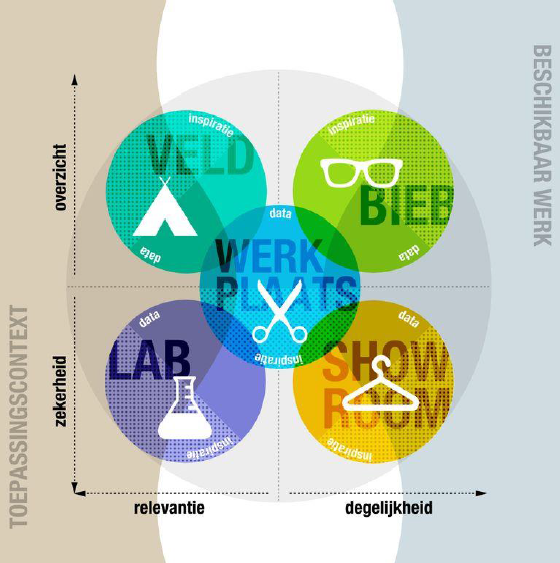
\includegraphics[width=0.5\linewidth]{Methodenkaart}\end{center}
	\label{fig:methodenkaart}
	\caption{De vijf werkplaatsen binnen het framework en hun systematiek. Overgenomen uit \textit{De informatieprofessional 3.0}  van \protect\citeA{MethodenKaart}  }
\end{figure}

\subsection{De gekozen onderzoeksmethodes}

De deelvragen gaan gedeeltelijk over keuzes van gebruik. 
Welke software en hardware is geschikt, is een vraag die veel naar voren komt.
Hieruit valt te concluderen dat de onderzoeker zich nog aan het oriënteren is.
"De onderzoeksruimte bieb bevat een verzameling methoden en technieken die dienen tot oriëntatie op beschikbaar werk."\cite{MethodenKaart}
Daarom wordt er gekozen om een bieb onderzoek uit te voren naar de deelvragen die gaan over geschiktheid.
Dit zodat de onderzoeker zich nog kan oriënteren naar het beschikbare aanbod en nog op nieuwe deelvragen kan komen. 

Lab onderzoek wordt pas later uitgevoerd omdat niet alle hardware voor handen is, maar ook omdat er niet genoeg tijd beschikbaar voor is.
\citeauthor{MethodenKaart} zegt het volgende over lab onderzoek: De onderzoeksruimte lab bevat methoden die geschikt zijn om de oplossing te toetsen aan een aspect van de toepassingscontext.
Daarom is het lab onderzoek geschikt voor het moment waarop de hardware beschikbaar is en de onderzoeker het gedrag hiervan exact in kaart wil brengen en wil bewijzen dat de gestelde eisen behaald worden.

\citeA{ICAoates} stelt dat een systeem bouwen 'bewijs' is dat een nieuw soort toepassing gebouwd kan worden. Als dit het doel is heeft het onderzoek waarschijnlijk hoofdzakelijk een werkplaats karakter, maar alle andere onderzoeksruimtes kunnen een rol spelen.
Gedurende het huidige onderzoek zal er door de onderzoeker software geschreven worden om bewijs te leveren dat een nieuw drone systeem een toepasbaar alternatief is.
Daarom past de werkplaats onderzoeksruimte goed bij dit onderzoek.


\section{Invloed op het project}



\chapter{Criteria}
\label{chapter:criteria}
Maak hier een lijst met criteria aan de hand van de hoofd- en deelvragen.
\begin{itemize}	
\item Zijn de criteria duidelijk opgesteld?
\item Waar moet de oplossing aan voldoen, staat dit erin?
\end{itemize}
\hrule

In \autoref{tab:criteria} worden codes gebruikt als naam voor de criteria, wat deze betekenen wordt eerst toegelicht:
\begin{itemize}
	\item ALG: Een algemene eis die in elke onderzoek meegenomen moet worden.
	\item SK: Een eis die gesteld worden in de keuze naar simulatie software.
	\item DR: Een eis voor de te gebruiken drone in de simulatie.
	\item PH: Eisen opgesteld aan het hardware prototype.
\end{itemize}

\begin{longtable}{|l|l|l|}
	\hline
	\rowcolor[HTML]{C0C0C0} 
	Naam & Beschrijving \\ \hline
	%\endfirsthead
	%
	\endhead
		\hypertarget{alg1}{ALG1}	&Is voorzien van API documentatie.        \\ \hline
		\hypertarget{alg2}{ALG2}	&Ondersteunt aansturing vanuit C++ .    \\ \hline
		\hypertarget{alg3}{ALG3}	&\begin{tabular}[c]{@{}l@{}}Heeft ondersteuning voor het Linux platform Ubuntu 18.04\end{tabular}        \\ \hline
		\hypertarget{alg4}{ALG4}	&Software is gratis in gebruik voor studenten        \\ \hline
		\hypertarget{sk1}{SK1}		&\begin{tabular}[c]{@{}l@{}}Heeft ondersteuning voor UAV (unmanned air vehicle) ook wel drone genoemd\end{tabular} \\ \hline
		\hypertarget{sk2}{SK2}		&\begin{tabular}[c]{@{}l@{}}Ondersteunt de simulatie van locatie bepaling sensoren zoals GPS.\end{tabular}        \\ \hline
		\hypertarget{sk3}{SK3}		&\begin{tabular}[c]{@{}l@{}}Heeft een kant en klare oplossing voor simulatie van externe krachten zoals wind.\end{tabular}        \\ \hline
		\hypertarget{sk4}{SK4}		& Heeft een ingebouwde pathfinding oplossing.        \\ \hline
		\hypertarget{sk5}{SK5}		& Ondersteunt ROS als middleware.        \\ \hline
		\hypertarget{sk6}{SK6}		& Ondersteunt de detectie van botsingen.        \\ \hline
		\hypertarget{sk7}{SK7}		& Ondersteunt de simulatie 100 drones tegelijk.        \\ \hline
		DR1		& De drone is een quadcopter.        \\ \hline
		DR2		& De drone is is voorzien van een API voor aansturing op basis van coördinaten.       \\ \hline
		DR3		& De API sluit aan op de middleware ROS.        \\ \hline
		DR4		& De drone is bruikbaar binnen de gekozen simulatie software.        \\ \hline%TODO gekozen software toevoegen
		DR5		& De drone moet een kleine goedkope drone representeren.        \\ \hline
		PH1		& Ondersteunt een bereik van minimaal 100 meter tot 1000 meter.  \\ \hline
		PH2		& Ondersteunt het gebruik van grid networking om tot een mesh te kunnen komen.  \\ \hline
		PH3		& Maakt gebruik van een openbare bandbreedte.\\ \hline
		PH4		& De antenne mag niet meer dan 10 euro kosten. \\ \hline
		PH5		& Moet zuinig in gebruik van stroom zijn. TODO beter defineren \\ \hline
		PS1		& Ondersteund een mesh netwerk van minimaal 100 nodes. \\ \hline
		PS2		& Het netwerk is zelf herstellend. \\ \hline
		PS3		& Ondersteund het draaien op een raspberry pi of een ardunio (UNO of NANO). \\ \hline
		PS4		& Ondersteund het versturen van zelfgemaakte berichten. \\ \hline
		
	\caption{Opgestelde criteria}
	\label{tab:criteria}
\end{longtable}

\chapter{Literatuur}


\section{Welke simulatie software is geschikt om een drone in na te bootsen?}

Voor het onderzoek wordt gebruik gemaakt van een simulatie omgeving.
Welke software wordt gebruik staat vastgesteld in deze paragraaf.
De keuze van software wordt bepaald door het uitvoeren van de bieb onderzoeksmethode. 
In de \autoref{tab:criteria} staan de criteria toegelicht waar de simulatie software aan moet voldoen.
Als hoofdcriteria wordt een lijst opgesteld met simulatoren die ondersteuning hebben voor ROS.
Vervolgens worden deze aan de hand van een kruistabel onderworpen aan de andere criteria.
Deze techniek is gebaseerd op de "Comparison Chart" van \cite{CMDmethod} uit de "\textit{CMD Methods Pack}"

De kandidaten zijn:
\begin{itemize}
	\item \href{https://www.energid.com/actin}{Actin} is een simulatie framework van het bedrijf Energid. Het is in staat om de beweging van verschillende robots gelijktijdig aan te sturen.
	\item \href{http://gazebosim.org/}{Gazebo} is een opensource robot simulatie framework bijzonder geschikt voor het simuleren van robotica in outdoor omgevingen door de uitgebreide Physics Engine Support.
	\item \href{http://www.coppeliarobotics.com/}{V-REP (Virtual Robot Experimentation Platform)} is een platform geschikt voor het snel bouwen van robot prototypes.
	\item \href{https://cyberbotics.com/}{Webots} is een open source-ontwikkelomgeving die wordt gebruikt voor het modelleren, programmeren en simuleren van mobiele robots.
	\item \href{http://openrave.org/}{OpenRAVE} biedt een ontwikkelomgeving voor het testen van motion planning algoritmes aan de hand van simulaties.
\end{itemize}

\begin{table}[H]
	\centering
	\begin{tabular}{l|*{10}r}
		%\backslashbox{Input}{Output} & int8\_t & int16\_t & int32\_t & uint8\_t & uint16\_t & uint32\_t \\
		\diagbox[width=2.7cm, height=2.4cm]{\raisebox{5pt}{\hspace*{0.25cm}Simulator}}{\raisebox{-1.27cm}{\rotatebox{90}{Eis}}} & \raisebox{-0.25cm}{\rotatebox{90}{\hyperlink{alg1}{ALG1}}} & \raisebox{-0.25cm}{\rotatebox{90}{\hyperlink{alg2}{ALG2}}} & \raisebox{-0.25cm}{\rotatebox{90}{\hyperlink{alg3}{ALG3}}} & \raisebox{-0.25cm}{\rotatebox{90}{\hyperlink{alg4}{ALG4}}} &
		\raisebox{-0.25cm}{\rotatebox{90}{\hyperlink{sk1}{SK1}}} & \raisebox{-0.25cm}{\rotatebox{90}{\hyperlink{sk2}{SK2}}} &
		\raisebox{-0.25cm}{\rotatebox{90}{\hyperlink{sk3}{SK3}}} & \raisebox{-0.25cm}{\rotatebox{90}{\hyperlink{sk4}{SK4}}} &
		\raisebox{-0.25cm}{\rotatebox{90}{\hyperlink{sk5}{SK5}}} & \raisebox{-0.25cm}{\rotatebox{90}{\hyperlink{sk6}{SK6}}} \\
		\midrule\\
		\hspace*{0.25cm}Actin 	& \checkmark & \checkmark 	& \checkmark & x 		  & \checkmark & x 			& \checkmark & x 		  &\checkmark & \checkmark	\\ \\
		\hspace*{0.25cm}Gazebo 	& \checkmark & \checkmark 	& \checkmark & \checkmark & \checkmark & \checkmark & \checkmark & \checkmark &\checkmark & \checkmark	\\ \\
		\hspace*{0.25cm}V-REP 	& \checkmark & x 			& \checkmark & \checkmark & \checkmark & \checkmark & \checkmark & \checkmark &\checkmark & x	\\ \\
		\hspace*{0.25cm}Webots 	& \checkmark & \checkmark 	& \checkmark & \checkmark & \checkmark & \checkmark & \checkmark & \checkmark &\checkmark & \checkmark 	\\ \\
		\hspace*{0.25cm}OpenRAVE& \checkmark & \checkmark	& \checkmark & \checkmark & x 		   & \checkmark & \checkmark & \checkmark &\checkmark & x 	\\ \\
		\bottomrule
	\end{tabular}%
	\caption{Kruistabel simulatiekeuze}
	\label{tab:kruissimkeuze}%
\end{table}%

In de \autoref{tab:kruissimkeuze} komt de simulatie software van Gazebo en Webots naar voren als enige simulatoren die voldoen aan de gestelde eisen.
Het nu zaak om te uit te zoeken welke van de twee het meest geschikt is voor het uitvoeren van dit onderzoek.

\subsection{Gazebo of Webots?}
In januari 2018 hebben \citeauthor{RobotCompare} een publicatie geschreven waarin zij drie simulatoren vergelijken in het aanbod van features en performance. 
Zij hebben een vergelijking gedaan tussen V-REP, Gazebo en ARGoS. 
ARGoS is niet meegenomen in de overweging omdat het geen ondersteuning heeft voor ROS.

In de conclusie van de publicatie komt Webots als het meest gebruiksvriendelijk naar voren in het gebruik en is in het bezit van de meeste features.
Het grote nadeel van Webots is dat het veel kracht vraagt van de computer waardoor het niet geschikt is voor de simulatie van veel drones tegelijk.

Daarmee komt de keuze uit op Gazebo. 
De resultaten van in de publicatie van \citeA{RobotCompare} tonen aan dat de software in staat is om veel drones tegelijk aan te kunnen sturen.
\citeA{RobotCompare} geeft als nadeel aan Gazebo dat de software niet in staat is om 3d meshes te manipuleren, de user interface niet inovatief is en Gazebo soms problemen met dependencies door de veschillende versies van ROS.
Dit laatste brengt een risico met zich mee voor het onderzoek daarom is het ook zaak dat dit als criteria meegenomen word in de deelvraag van \autoref{sec:dronekeuze} \nameref{sec:dronekeuze}. 

\subsection{Conclusie}
Voor het onderzoek wordt Gazebo gebruikt omdat het voldoet aan de gestelde \nameref{chapter:criteria}.
De meest recente versie van Gazebo, die niet meer beta is op 19 februari 2019, is Gazebo 9.
Deze versie vereist het gebruik van ROS Melodic volgens haar eigen website  (\href{http://gazebosim.org/tutorials?tut=ros_wrapper_versions}{zie link}).

\section{Welke gesimuleerde drone is geschikt voor de simulatie software?}
\label{sec:dronekeuze}

\chapter{Oplossingsrichtingen}

\begin{itemize}
\item Beschrijf je hoe jouw oplossingsrichting de hoofdvraag beantwoord?
\item Beschrijft de oplossingsrichting de mogelijkheden?
\item Staat hier "Veld" vermeldt van de methodekaart van de HAN?
\end{itemize}
\hrule

\chapter{Experimenten}

\begin{itemize}
\item Beschrijft waarom dit experiment van belang is.
\item Voldoet de code van het experiment aan de opgestelde eisen?
\item Voldoet het programma aan de opgestelde QoS?
\item Is gedocumenteerd waarom het programma voldoet aan de opgestelde eisen?
\item Is gedocumenteerd waarom het programma voldoet aan de opgestelde QoS?
\end{itemize}
\hrule

\chapter{Conclusie}

\label{chapter:conclusie}
Conclusie uit resultaten. Herhaal en beantwoord de hoofdvraag.
\begin{itemize}
\item Trek een conclusie uit de resultaten van de deelvragen.
\item Wordt de hoofdvraag beantwoord?
\item Wat beveel je aan?
\end{itemize}
\hrule


\bibliographystyle{apacite}
\bibliography{bilbliography.bib}

\clearpage
\appendix

\end{document}